\chapter{\ifenglish Background Knowledge and Theory\else ทฤษฎีที่เกี่ยวข้อง\fi}

\section{รถรับส่งไฟฟ้าของขนส่งมวลชนมหาวิทยาลัยเชียงใหม่}
  รถรับส่งไฟฟ้าขนาด 16 ที่นั่ง (ไม่รวมคนขับ) 2 ประตู (ไม่รวมประตูฝั่งคนขับ) ที่ให้บริการนักศึกษาและบุคลากรของมหาวิทยาลัยเชียงใหม่ในการไปยังสถานที่ต่างๆระหว่างมหาวิทยาลัยเชียงใหม่
  \begin{figure}[h!]
    \begin{center}
      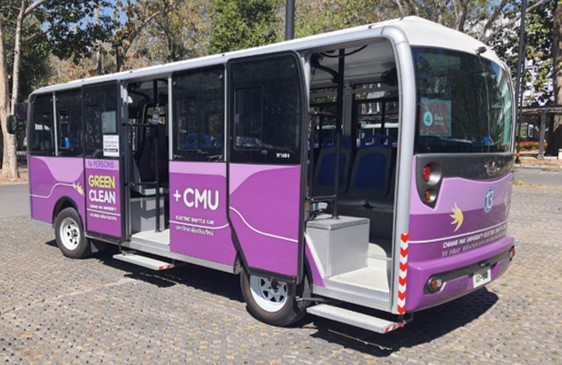
\includegraphics[width=0.5\textwidth]{cmu-evbus.jpg}
    \end{center}
    \caption[Poem]{รถรับส่งไฟฟ้าของขนส่งมวลชนมหาวิทยาลัยเชียงใหม่}
    \label{fig:cmu-ebus}
  \end{figure}

\section{อุปกรณ์วัดระยะห่างโดยใช้อินฟราเรด Sharp GP2Y0A02YK0F}
  \cite[อุปกรณ์วัดระยะห่างโดยใช้อินฟราเรด Sharp GP2Y0A02YK0F]{sharpgp2y0a02yk0f} เป็นอุปกรณ์สำหรับวัดระยะห่างระหว่างตัวอุปกรณ์และวัตถุที่อยู่หน้าอุปกรณ์ ซึ่งการรวมกันของอุปกรณ์ตรวจจับตำแหน่งแสง หรือ Position Sensitive Detector (PSD), ไอโอดแบบเปล่งแสงอินฟราเรด และวงจรประมวลผลสัญญาณหรือ Signal Processing Unit โดยไอโอดแบบเปล่งแสงอินฟราเรด จะเปล่งแสงอินฟราเรดออกไป หากมีวัตถุมาขวางทางของแสง แสงจะสะท้อนกลับมายังอุปกรณ์ตรวจจับตำแหน่งแสงแล้วส่งสัญญาณไปยังวงจรประมวลผลสัญญาณ โดยข้อมูลระยะทางจะส่งในรูปแบบของแรงดันไฟฟ้า ยิ่งวัตถุอยู่ใกล้ จะมีแรงดันไฟฟ้าสูง โดยอุปกรณ์วัดระยะห่างโดยใช้อินฟราเรด Sharp GP2Y0A02YK0F จะสามารถวัดระยะห่างของวัตถุที่มีสีได้ตั้งแต่ 20 เซนติเมตร ไปจนถึง 150 เซนติเมตร
  \begin{figure}[h!]
    \begin{center}
      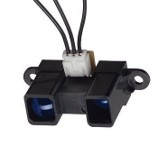
\includegraphics[width=0.25\textwidth]{Sharp-GP2Y0A02YK0F.jpg}
    \end{center}
    \caption[Poem]{อุปกรณ์วัดระยะห่างโดยใช้อินฟราเรด Sharp GP2Y0A02YK0F}
    \label{fig:Sharp-GP2Y0A02YK0F}
  \end{figure}

\section{อุปกรณ์รับ-ส่งข้อมูล GNSS u-blox Neo-7M}
  \cite[อุปกรณ์รับ-ส่งข้อมูล GNSS u-blox Neo-7M]{u-blox-neo-7m} เป็นอุปกรณ์สำหรับรับ-ส่งข้อมูลตำแหน่งทาง GNSS (GPS, GLONASS, QZSS และ SBAS) 
  \begin{figure}[h!]
    \begin{center}
      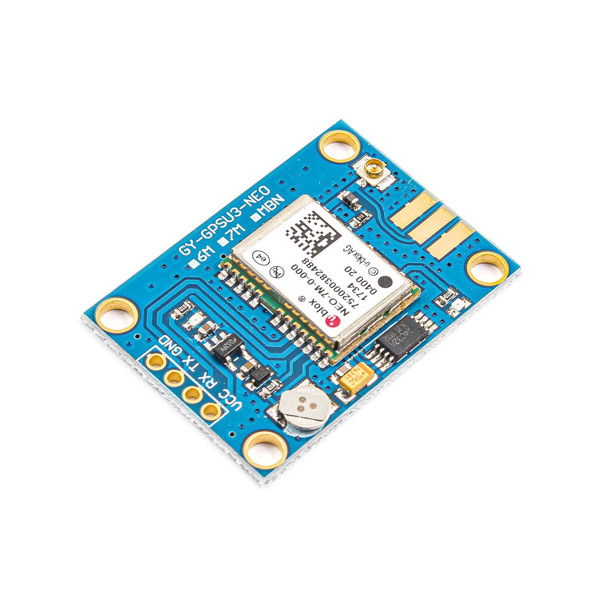
\includegraphics[width=0.25\textwidth]{u-blox-neo-7m.jpg}
    \end{center}
    \caption[Poem]{อุปกรณ์รับ-ส่งข้อมูล GNSS u-blox Neo-7M}
    \label{fig:u-blox-neo-7m}
  \end{figure}

 \section{ไมโครคอรโทรลเลอร์ ESP32}
  \cite[ไมโครคอรโทรลเลอร์ ESP32]{esp32} เป็นไมโครคอนโทรลเลอร์ที่สามารถเชื่อมต่อเครือข่ายไวไฟและบลูทูธได้ และมีความสามารถในการเชื่อมต่อกับอุปกรณ์อื่นๆ ได้หลากหลาย โดยไมโครคอรโทรลเลอร์ ESP32 สามารถเชื่อมต่อกับอุปกรณ์อื่นๆ ผ่านทางอินเทอร์เฟซต่างๆ ได้ เช่น อินเทอร์เฟซ UART, SPI, I2C, GPIO, ADC, DAC, PWM ฯลฯ รวมไปถึงสามารถเขียนโปรแกรมเพื่อควบคุมได้ ทำให้ไมโครคอรโทรลเลอร์ ESP32 มีความสามารถในการทำงานต่างๆ ได้หลากหลาย
  \begin{figure}[h!]
    \begin{center}
      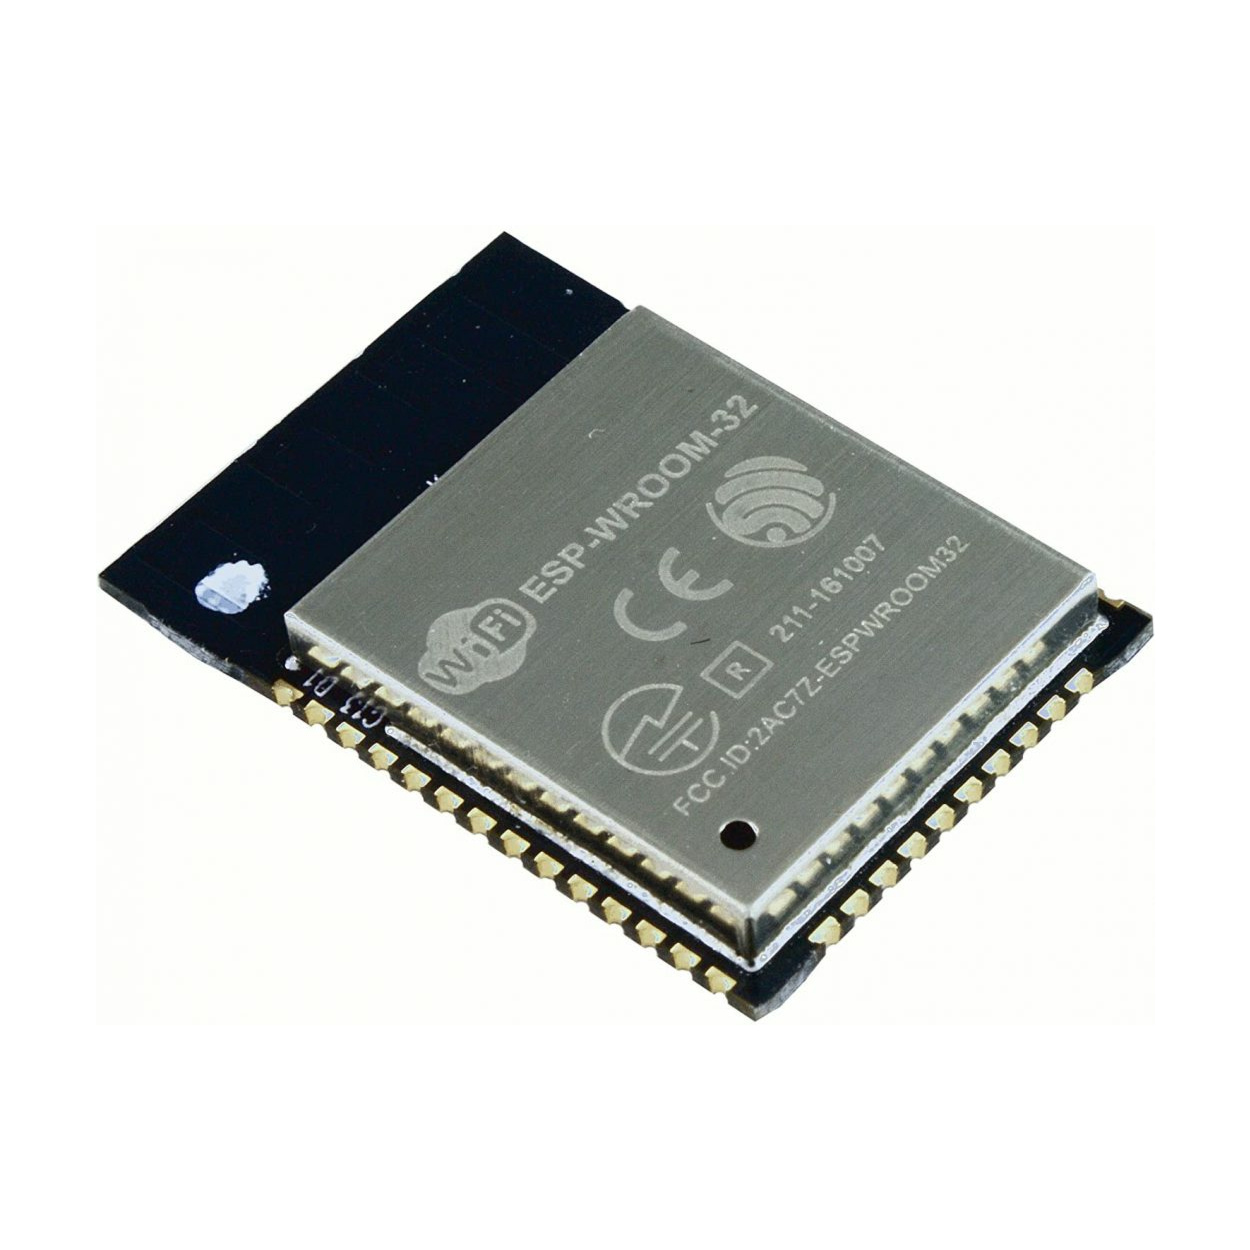
\includegraphics[width=0.25\textwidth]{esp32.png}
    \end{center}
    \caption[Poem]{ไมโครคอรโทรลเลอร์ ESP32}
    \label{fig:esp32}
  \end{figure}

\section{โมเด็ม SIMCOM A7608}
  โมเด็ม SIMCOM A7608 เป็นโมเด็มสำหรับการเชื่อมต่อเครือข่ายไร้สายทั้ง 4G และไวไฟ รวมไปถึงมีอินเตอร์เฟสสำหรับเชื่อมต่อกับโปรโตคอลต่างๆได้ อาทิ MQTT, HTTP ฯลฯ ทำให้สามารถใช้งานโมเด็ม SIMCOM A7608 ในการส่งข้อมูลไปยังเซิร์ฟเวอร์ได้ผ่าน AT Command
  \begin{figure}[h!]
    \begin{center}
      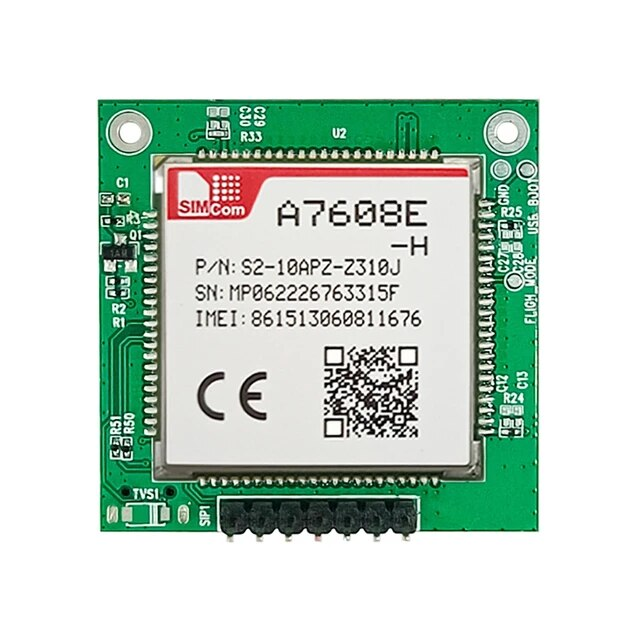
\includegraphics[width=0.25\textwidth]{simcom-a7608e-h.png}
    \end{center}
    \caption[Poem]{โมเด็ม SIMCOM A7608}
    \label{fig:simcom-a7608}
  \end{figure}

\section{บอร์ดสำหรับพัฒนา LILYGO T-A7608}
  บอร์ดสำหรับพัฒนา LILYGO T-A7608 เป็นบอร์ดสำหรับพัฒนาที่รวมเอาความหลากหลายในการทำงานของไมโครคอนโทรลเลอร์ ESP32 และความสามารถในการเชื่อมต่อเครือข่ายไร้สายของ โมเด็ม SIMCOM A-7608 เข้าด้วยกัน ทำให้สามารถใช้งานทั้งสองอุปกรณ์ในการทำงานร่วมกันได้ผ่าน Library ที่ผู้พัฒนาจัดเตรียมไว้ให้
  \begin{figure}[h!]
    \begin{center}
      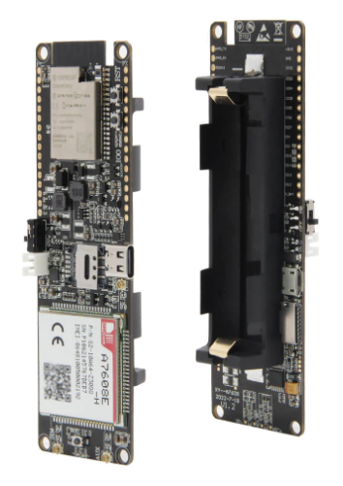
\includegraphics[width=0.25\textwidth]{lilygo-t-a7608.png}
    \end{center}
    \caption[Poem]{บอร์ดสำหรับพัฒนา LILYGO T-A7608}
    \label{fig:lilygo-t-a7608}
  \end{figure}

\section{เครือข่าย LTE}
  \cite[เครือข่าย LTE (Long Term Evolution)]{lte} เป็นเครือข่ายสื่อสารไร้สายที่ใช้ในการสื่อสารข้อมูลระหว่างอุปกรณ์ไร้สาย โดยเครือข่าย LTE สามารถให้ความเร็วในการส่งข้อมูลได้สูงถึง 100 Mbps ในการส่งข้อมูล และ 50 Mbps ในการรับข้อมูล ทำให้เครือข่าย LTE มีความเร็วในการส่งข้อมูลที่สูงกว่าเครือข่ายอื่นๆ ที่ใช้ในการสื่อสารข้อมูลระหว่างอุปกรณ์ไร้สาย รวมไปถึงในปัจจุบัน เครือข่าย LTE ครอบคลุมมากพอที่จะใช้งานในชีวิตแระจำวัน รวมถึงในการพัฒนาโครงงานได้

\section{Global Positioning System}
  Global Positioning System หรือ GPS เป็นระบบดาวเทียมนำร่องโลก เพื่อระบุข้อมูลของตำแหน่งและเวลาโดยอาศัยการคำนวณจากความถี่สัญญาณนาฬิกาที่ส่งมาจากตำแหน่งของดาวเทียมต่างๆ ที่โคจรอยู่รอบโลกทำให้สามารถระบุตำแหน่ง ณ จุดที่สามารถรับสัญญาณได้ทั่วโลกและในทุกสภาพอากาศ รวมถึงสามารถคำนวณความเร็วและทิศทางเพื่อนำมาใช้ร่วมกับแผนที่ในการนำทางได้

\section{โปรโตคอลการส่งข้อมูล HTTP}

\section{โปรโตรคอลการส่งข้อความ MQTT}
  MQTT เป็นโปรโตคอลการส่งข้อความที่อิงตามมาตรฐาน หรือชุดของกฎที่ใช้สําหรับการสื่อสารระหว่าง เครื่องต่อเครื่อง เซ็นเซอร์อัจฉริยะ อุปกรณ์สวมใส่ และอุปกรณ์Internet of Things (IoT) อื่นๆ มักจะ ต้องส่งและรับข้อมูลผ่านเครือข่ายที่มีข้อจํากัดด้านทรัพยากร ซึ่งมีแบนด์วิดท์จํากัด อุปกรณ์IoT เหล่านี้ใช้ MQTT ในการรับส่งข้อมูล เนื่องจากมันใช้งานง่ายและสามารถสื่อสารข้อมูล IoT ได้อย่างมีประสิทธิภาพ MQTT รองรับการส่งข้อความจากอุปกรณ์ไปยังคลาวด์และจากคลาวด์ไปยังอุปกรณ์

\section{โปรโตคอลการส่งข้อความ REST}
  Representational State Transfer (REST) เป็นสถาปัตยกรรมซอฟต์แวร์ที่กําหนดเงื่อนไขว่า API ควร ทํางานอย่างไร โดยแต่แรกเริ่มนั้น มีการสร้าง REST ขึ้นเพื่อเป็นแนวทางในการจัดการการสื่อสารบนเครือ ข่ายที่ซับซ้อน เช่น อินเทอร์เน็ต คุณสามารถใช้สถาปัตยกรรม REST เพื่อรองรับการสื่อสารที่มีประสิทธิภาพ สูงและเชื่อถือได้ในทุกระดับ คุณยังสามารถใช้และปรับเปลี่ยนสถาปัตยกรรมได้อย่างง่ายดาย โดยนําความสามารถในการมองเห็นและการเคลื่อนย้ายข้ามแพลตฟอร์มมาสู่ทุกระบบ API

\section{โบรกเกอร์ MQTT Mosquitto}

\section{Node.js}

\section{influxDB}

\section{React.js}

\section{DigitalOcean Droplet}

\section{\ifenglish%
\ifcpe CPE \else ISNE \fi knowledge used, applied, or integrated in this project
\else%
ความรู้ตามหลักสูตรซึ่งถูกนำมาใช้หรือบูรณาการในโครงงาน
\fi
}
\begin{itemize}
  \item 261102 Computer Programming - พื้นฐานการเขียนโปรแกรมคอมพิวเตอร์
  \item 261207 Basic Computer Engineering Laboratory - พื้นฐานการเขียนเว็บแอพพลิเคชันและการส่งข้อมูล
  \item 252281 Fundamental of Electronics Circuits for ISNE, 261210 Logic and Digital Circuits - การวิเคราห์และออกแบบวงจรดิจิทัล
  \item 261214 Microprocessor and Interfacing - การเขียนโปรแกรมไมโครคอนโทรลเลอร์
  \item 261342 Fundamentals of Database Systems - พื้นฐานการออกแบบและใช้งานฐานข้อมูล
  \item 261441 Internet of Things and Big Data - การส่งข้อมูลและรูปแบบการส่งข้อมูลระหว่างอุปกรณ์อินเตอร์เน็ตในทุกสรรพสิ่งและเครือข่าย
\end{itemize}

\section{\ifenglish%
Extracurricular knowledge used, applied, or integrated in this project
\else%
ความรู้นอกหลักสูตรซึ่งถูกนำมาใช้หรือบูรณาการในโครงงาน
\fi
}
\begin{itemize}
  \item การใช้งานบอร์ดสำหรับพัฒนา LILYGO T-A7608
  \item การใช้งานอุปกรณ์รับ-ส่งข้อมูล GNSS u-blox Neo-7M
  \item การออกแบบระบบบนคลาวด์ที่ใช้ระบบปฏิบัติการ Ubuntu รวมไปถึงการให้บริการระบบต่างๆบนคลาวด์
\end{itemize}

